\documentclass[12pt,letterpaper]{article}
\usepackage{graphicx,textcomp}
\usepackage{natbib}
\usepackage{setspace}
\usepackage{fullpage}
\usepackage{color}
\usepackage[reqno]{amsmath}
\usepackage{amsthm}
\usepackage{fancyvrb}
\usepackage{amssymb,enumerate}
\usepackage[all]{xy}
\usepackage{endnotes}
\usepackage{lscape}
\newtheorem{com}{Comment}
\usepackage{float}
\usepackage{hyperref}
\newtheorem{lem} {Lemma}
\newtheorem{prop}{Proposition}
\newtheorem{thm}{Theorem}
\newtheorem{defn}{Definition}
\newtheorem{cor}{Corollary}
\newtheorem{obs}{Observation}
\usepackage[compact]{titlesec}
\usepackage{dcolumn}
\usepackage{tikz}
\usetikzlibrary{arrows}
\usepackage{multirow}
\usepackage{xcolor}
\newcolumntype{.}{D{.}{.}{-1}}
\newcolumntype{d}[1]{D{.}{.}{#1}}
\definecolor{light-gray}{gray}{0.65}
\usepackage{url}
\usepackage{listings}
\usepackage{color}

\definecolor{codegreen}{rgb}{0,0.6,0}
\definecolor{codegray}{rgb}{0.5,0.5,0.5}
\definecolor{codepurple}{rgb}{0.58,0,0.82}
\definecolor{backcolour}{rgb}{0.95,0.95,0.92}

\lstdefinestyle{mystyle}{
	backgroundcolor=\color{backcolour},   
	commentstyle=\color{codegreen},
	keywordstyle=\color{magenta},
	numberstyle=\tiny\color{codegray},
	stringstyle=\color{codepurple},
	basicstyle=\footnotesize,
	breakatwhitespace=false,         
	breaklines=true,                 
	captionpos=b,                    
	keepspaces=true,                 
	numbers=left,                    
	numbersep=5pt,                  
	showspaces=false,                
	showstringspaces=false,
	showtabs=false,                  
	tabsize=2
}
\lstset{style=mystyle}
\newcommand{\Sref}[1]{Section~\ref{#1}}
\newtheorem{hyp}{Hypothesis}

\title{PS Response: Problem Set 1}
\date{Sein Kim}
\author{Applied Stats/Quant Methods 1}

\begin{document}
		\maketitle
	
		\vspace{1cm}
\section*{Question 1: Education}
	
				A school counselor was curious about the average of IQ of the students in her school and took a random sample of 25 students' IQ scores. The following is the data set:\\
				\vspace{.5cm}
				
				\lstinputlisting[language=R, firstline=36, lastline=36]{PS01_SK.R}  
				
				\vspace{1cm}
				
				\begin{enumerate}
					\item Find a 90\% confidence interval for the average student IQ in the school.
					
					\lstinputlisting[language=R, firstline=39, lastline=51]{PS01_SK.R}
					
					\vspace{.25cm}
					
					  \begin{verbatim}
						> print(round(mean_y,2))
						[1] 98.44
						> print(round(n,2))
						[1] 25
						> print(round(s,2))
						[1] 13.09
						> print(round(SE, 2))
						[1] 2.62
						> print(round(tcrit_1,2))
						[1] 1.71
						> print(round(ci_90_lower,2))
						[1] 93.96
						> print(round(ci_90_upper,2))
						[1] 102.92
					\end{verbatim}
					\lstinputlisting[language=R, firstline=53, lastline=54]{PS01_SK.R}
					 \vspace{.25cm}
					   \noindent The sample mean was $98.44$ with $n=25$, $s=13.09$, and standard error $2.62$.
					Using a $t$-distribution with $df = 24$ and $t_{\text{crit, }0.95,24} = 1.71$, 
					the 90\% confidence interval for the average IQ in the school is:
					\[
					(93.96,\; 102.92).
					\]
				
					\item Next, the school counselor was curious  whether  the average student IQ in her school is higher than the average IQ score (100) among all the schools in the country.
					
					\noindent Using the same sample, conduct the appropriate hypothesis test with $\alpha=0.05$.
					
					\lstinputlisting[language=R, firstline=69, lastline=72]{PS01_SK.R}
					
						\begin{verbatim}
						> print(round(n, 2))
						[1] 25
						> print(round(mean_y, 2))
						[1] 98.44
						> print(round(s, 2))
						[1] 13.09
						> print(round(SE, 2))
						[1] 2.62
						> print(round(t_stat, 2))
						[1] -0.6
						> print(round(t_crit, 2))
						[1] 1.71
						> print(round(p_value, 2))
						[1] 0.72
						\end{verbatim}
				
					\noindent I conducted a one-sided t-test with $H_0:\mu=100$ and $H_1:\mu>100$. The sample mean was 98.44 with $n=25$, $s=13.09$, and standard error 2.62. The test statistic was $t=-0.596$, the critical value at $\alpha=0.05$ was 1.711, and the one-sided p-value was 0.72. Since $p > 0.05$, we fail to reject the null hypothesis and conclude that there is no statistical evidence that the school mean IQ is greater than 100.
					
					\noindent Or, I can simply use \textbf{\textit{t.test}} function to get an answer.
				
					\lstinputlisting[language=R, firstline=79, lastline=79]{PS01_SK.R}	
					\begin{verbatim}
						One Sample t-test
						
						data:  y
						t = -0.59574, df = 24, p-value = 0.7215
						alternative hypothesis: true mean is greater than 100
						95 percent confidence interval:
						93.95993      Inf
						sample estimates:
						mean of x 
						98.44 
					\end{verbatim}
					
				\end{enumerate}

\section*{Question 2: Political Economy}

	\noindent Researchers are curious about what affects the amount of money communities spend on addressing homelessness. The following variables constitute our data set about social welfare expenditures in the USA. \\
	\vspace{.5cm}
	
	
	\begin{tabular}{r|l}
		\texttt{State} &\emph{50 states in US} \\
		\texttt{Y} & \emph{per capita expenditure on shelters/housing assistance in state}\\
		\texttt{X1} &\emph{per capita personal income in state} \\
		\texttt{X2} &  \emph{Number of residents per 100,000 that are "financially insecure" in state}\\
		\texttt{X3} &  \emph{Number of people per thousand residing in urban areas in state} \\
		\texttt{Region} &  \emph{1=Northeast, 2= North Central, 3= South, 4=West} \\
	\end{tabular}
	
	\vspace{.5cm}
	\noindent Explore the \texttt{expenditure} data set and import data into \texttt{R}.
	\vspace{.5cm}
	\lstinputlisting[language=R, firstline=89, lastline=90]{PS01_SK.R}  
							
	\vspace{.5cm}
	\begin{itemize}
	
	\item
	Please plot the relationships among \emph{Y}, \emph{X1}, \emph{X2}, and \emph{X3}? What are the correlations among them (you just need to describe the graph and the relationships among them)?
	\vspace{.5cm}
		
		\lstinputlisting[language=R, firstline=95, lastline=118]{PS01_SK.R}
		
		\begin{verbatim}
			> round(cor_mat, 3)
			Y    X1    X2    X3
			Y  1.000 0.532 0.448 0.464
			X1 0.532 1.000 0.206 0.595
			X2 0.448 0.206 1.000 0.221
			X3 0.464 0.595 0.221 1.000
			
			> cat("corr(Y, X1) =", round(cor_mat["Y","X1"], 3), "\n")
			corr(Y, X1) = 0.532 
			> cat("corr(Y, X2) =", round(cor_mat["Y","X2"], 3), "\n")
			corr(Y, X2) = 0.448 
			> cat("corr(Y, X3) =", round(cor_mat["Y","X3"], 3), "\n")
			corr(Y, X3) = 0.464
		\end{verbatim}
		
		\begin{figure}[H]\centering
			\caption{\footnotesize Pairwise scatterplots among $Y$, $X_1$, $X_2$, and $X_3$.}
			
\includegraphics[width=0.8\textwidth]{q2_pairs.pdf}
		\end{figure}
		
		\begin{figure}[H]\centering
			\caption{\footnotesize Scatterplots of $Y$ vs $X_1$, $X_2$, and $X_3$.}
			
\includegraphics[width=0.9\textwidth]{q2_Y_vs_Xs.pdf}
		\end{figure}
	
	\vspace{0.5cm}
	\noindent From the scatterplots and the Pearson correlation matrix, all relationships between $Y$ and $X_1$, $X_2$, and $X_3$ are positive. 
	The association between $Y$ and $X_1$ ($r=0.532$) is the strongest, indicating that states with higher per-capita income tend to spend more on housing assistance. 
	Meanwhile, $X_2$ (financial insecurity) and $X_3$ (urbanization) show moderate positive relationships with $Y$ ($r=0.448$ and $r=0.464$ respectively). 
	Overall, higher income and greater urbanization appear related to higher per-capita expenditure on housing assistance.
	\vspace{.5cm}
	
	\item
	Please plot the relationship between \emph{Y} and \emph{Region}? On average, which region has the highest per capita expenditure on housing assistance?

	
	\lstinputlisting[language=R, firstline=124, lastline=135]{PS01_SK.R}
	
	\begin{verbatim}
		> print(round(region_means,2))
			    1     2     3     4 
			79.44 83.92 69.19 88.31 
	\end{verbatim}
	
	\begin{figure}[H]\centering
		\caption{\footnotesize Boxplot of $Y$ by Region. Red points indicate regional means.}
		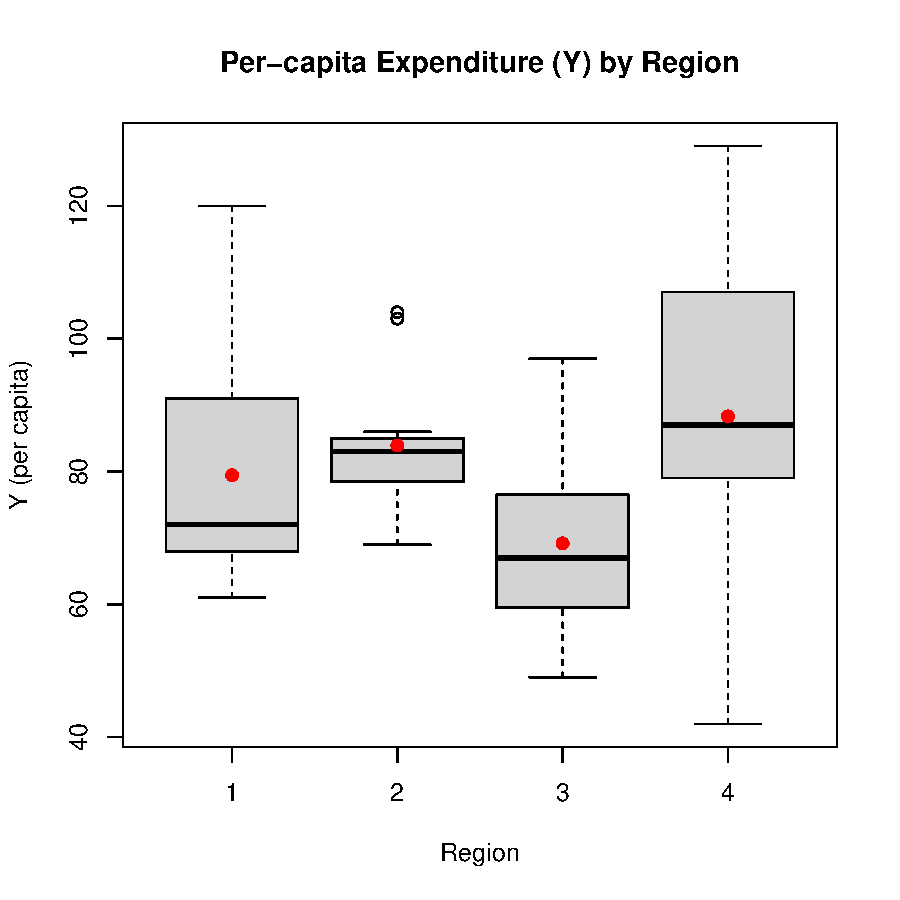
\includegraphics[width=0.65\textwidth]{q2_Y_by_region.pdf}
	\end{figure}

	
	\noindent I chose a \textbf{boxplot} because it clearly shows the distribution of $Y$ within each region, including the spread, median, and potential outliers, and allows for easy comparison across groups. The red dots represent the regional means, making it straightforward to identify which region spends the most. From the output, \textbf{Region 4 (West)} has the highest mean per-capita expenditure on housing assistance, while \textbf{Region 3 (South)} shows the lowest. This suggests that western states tend to allocate more resources to housing assistance compared to southern states.
	\vspace{.5cm}
	\item
	Please plot the relationship between \emph{Y} and \emph{X1}? Describe this graph and the relationship. Reproduce the above graph including one more variable \emph{Region} and display different regions with different types of symbols and colors.
	\vspace{.5cm}
	
	\lstinputlisting[language=R, firstline=142, lastline=166]{PS01_SK.R}
	
	\begin{figure}[H]\centering
		\caption{\footnotesize Scatterplot of $Y$ vs $X_1$ with fitted regression line.}
		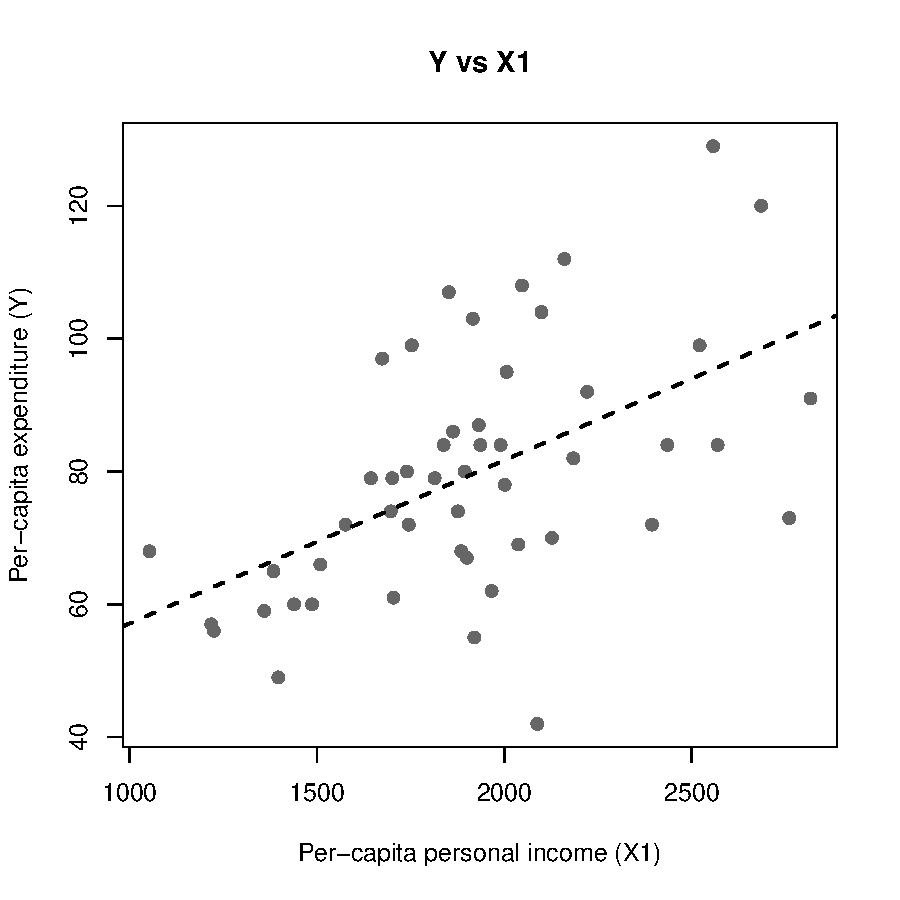
\includegraphics[width=0.65\textwidth]{q2_Y_vs_X1.pdf}
	\end{figure}
	
	\begin{figure}[H]\centering
		\caption{\footnotesize Scatterplot of $Y$ vs $X_1$ by Region. Colors and symbols distinguish regions.}
		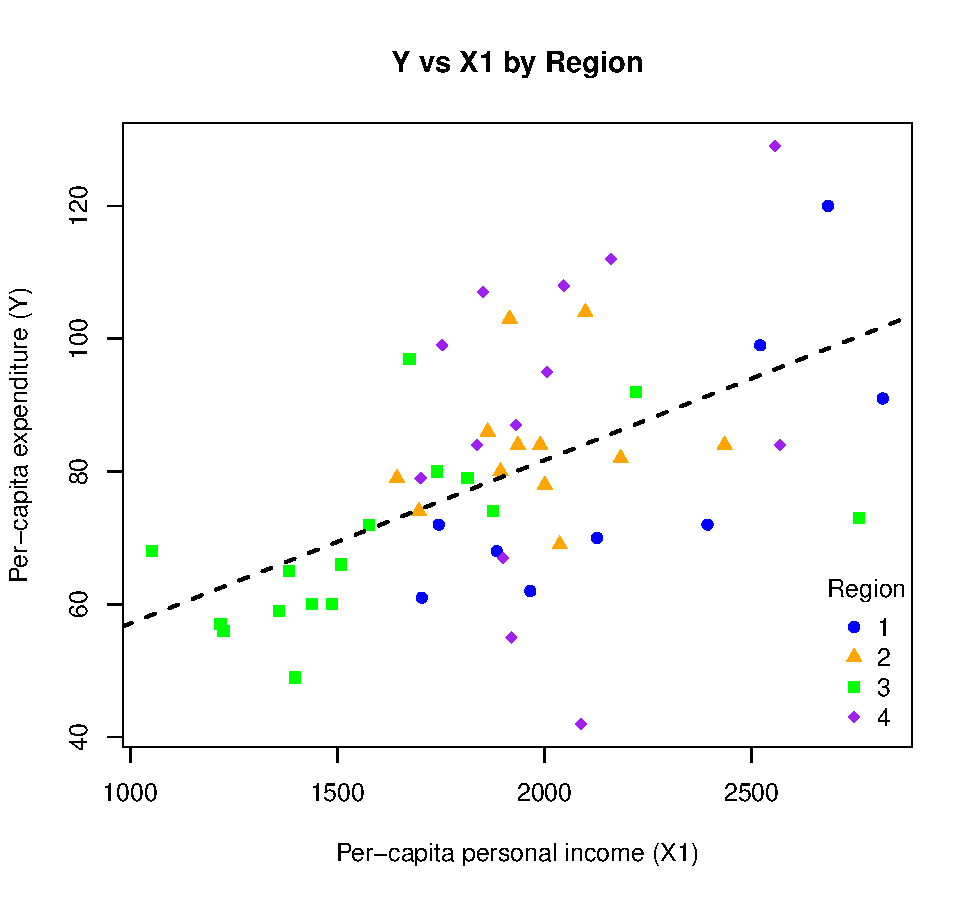
\includegraphics[width=0.70\textwidth]{q2_Y_vs_X1_by_region.pdf}
	\end{figure}
	
	\noindent The scatterplot of $Y$ versus $X_1$ shows a moderate positive relationship: states with higher per-capita income tend to spend more on housing assistance. When we add \emph{Region}, the points are distinguished by color and symbol, revealing that while the overall trend is positive, regional differences are also visible. In particular, \textbf{Region 4 (West)} and \textbf{Region 1 (Northeast)} generally cluster toward higher income and expenditure levels, whereas \textbf{Region 3 (South)} tends to have lower values for both.
	\end{itemize}
	
	\end{document}
